\documentclass[12pt]{extarticle}

\usepackage{preamble}
\usepackage{preamble_svg}
\usepackage{siunitx}

\title{Physics 2 Notes, Partial 2}
\date{Semester 2, 2023/2024}

\setlength{\headheight}{15pt} % ??? we do what fancyhdr tells us to do

% Units
\DeclareSIUnit\angstrom{Å} % Redefine it as it got deprecated
\DeclareSIUnit\atm{atm}
\DeclareSIUnit{\calorie}{cal}

\newcommand{\anglebraces}[1]{
    \langle #1 \rangle
}

\begin{document}

\firstpage

% Class of 21/03/2024
\section{Rotational Dynamics}

\subsection{Introduction}

We define a \emph{rigid body} as an object that never changes its shape.
Mathematically we can say that given any $i, j$ inside the body, the distance $d_{ij}$ will stay constant no matter what.

\subsubsection{Types of rigid bodies}

We can differentiate between continuos rigid body and discrete rigid bodies:
\begin{itemize}
    \item Continuous rigid bodies have a density mass function of the form $\rho(\vec{r})$.
    \item Discrete rigid bodies have a finite number of particles, each with a mass $m_i$ and a position $\vec{r}_i$, which might all be connected by some massless structure.
\end{itemize}

\subsubsection{Decomposing displacements}

We want to describe the motion of a rigid body in space. This is usually a hard task.

It turns out that a general displacement of a rigid body can be decomposed into the sum of two motions: a \textbf{translation} of the center of mass and a \textbf{rotation} around the center of mass.
This means that we need 6 parameters to describe any displacement: 3 for the translation and 3 for the rotation.

\subsubsection{The simplest case: 2D}

The simplest case we will consider is a 2D rigid body that lies on the $xy$ plane and can rotate around the $z$ axis.

\subsection{Angular variables}

Consider a simple case of a 2D rigid body that can rotate around the $z$ axis and has its center of mass fixed at the origin.

In this case we can describe the position of any point $p$ in the RB in polar coordinates as $(r, \theta)$. Now, knowing $r$ and $\theta$ we can compute the \textbf{arc length} $s = r\theta$.

Note that specifying $\theta$ is enough to get the position of all the points in the RB because $r$ will stay constant.

\subsubsection{Angular velocity}

Let $\omega_{\text{avg}} \coloneq \frac{\theta(t_2) - \theta(t_1)}{t_2 - t_1}$ be the \textbf{average angular velocity} between times $t_1$ and $t_2$. As $\Delta t = t_2 - t_1 \to 0$, we define the \textbf{instantaneous angular velocity} as

\begin{equation}
    \omega \coloneq \lim_{\Delta t \to 0} \omega_{\text{avg}} = \dv{\theta}{t}
\end{equation}

The angular velocity is a vector, therefore we can decompose it in direction and magnitude. We have $\vec{\omega} = \omega \hat{\omega}$, where $\hat{\omega}$ is either $\hat{z}$ if the motion is counterclockwise or $-\hat{z}$ if the motion is clockwise.

Moreover note that the angular velocity stays constant for every point in the RB, but the linear velocity does not, in fact $v = r\omega$.

\subsubsection{Angular acceleration}

We define the \textbf{average angular acceleration} as $\alpha_{\text{avg}} \coloneq \frac{\omega(t_2) - \omega(t_1)}{t_2 - t_1}$ and the \textbf{instantaneous angular acceleration} as

\begin{equation}
    \alpha \coloneq \lim_{\Delta t \to 0} \alpha_{\text{avg}} = \dv{\omega}{t} = \dv[2]{\theta}{t}
\end{equation}

If we want to calculate the linear acceleration of a point in the RB, we have to combine the centripetal acceleration and the tangential acceleration, that is

$$
    a = \begin{cases}
        a_c = \frac{v^2}{r} = r\omega^2 \\
        a_t = \dv{v}{t} = \dv{t}(\omega r) = r \dv{\omega}{t} = r\alpha
    \end{cases}
$$

\subsection{Rotational kinetic energy}

First we will consider a simpler case of a discrete rigid body of $n$ masses connected by a stick around a pivot which also happens to be the center of mass.

Then the kinetic energy $K = \sum_{i=1}^n K_i$ where

\begin{align}
    K_i & = \frac{1}{2}m_i v_i^2          \\
        & = \frac{1}{2}m_i r_i^2 \omega^2
\end{align}

note that the $i$ subscript is only present in the mass and the radius, but not in the angular velocity, then we can write

\begin{align}
    K & = \frac{1}{2} \omega^2 \sum_{i=1}^n m_i r_i^2 \\
      & = \frac{1}{2} I \omega^2
\end{align}

where $I \coloneq \sum_{i=1}^n m_i r_i^2$ is the \textbf{moment of inertia} of the rigid body.

\subsubsection{Moment of inertia}

We can make some trivial observations about the moment of inertia:

\begin{itemize}
    \item It depends on $m_i$ and $r_i$: if the RB is heavier or more spread out, the moment of inertia will be bigger.
    \item It depends on the axis of rotation: if we change the pivot point the moment of inertia will change because the $r_i$ will change.
\end{itemize}

In the case of a continuous rigid body, we can see it just as a sum of an infinite number of masses, so we can write

\begin{align}
    K & = \int_{RB} \dd{K}                          \\
      & = \int_{RB} \frac{1}{2} v^2 \dd{m}          \\
      & = \int_{RB} \frac{1}{2} r^2 \omega^2 \dd{m} \\
      & = \frac{1}{2} I \omega^2
\end{align}

where

\begin{equation}
    I \coloneq \int_{RB} r^2 \dd{m} = \int_{RB} r^2 \sigma \dd{S}
\end{equation}

where $\sigma$ is the density mass function on a surface.

Note that $r$ and $\sigma$ are functions of the position, even if we dropped the notation this does not mean that $I$ is a constant.

\begin{remark}
    For a matter of notation, we will use the symbol $\lambda$ to denote the linear density mass function, $\sigma$ to denote the surface density mass function and $\rho$ to denote the volume density mass function.
\end{remark}

\begin{example}[moment of inertia of a ring]
    Consider a ring of radius $R$ and mass $M$ with uniform density. We want to calculate the moment of inertia with respect to the center of the ring.

    Since the density is uniform, we can write $\lambda = \frac{M}{2\pi R}$, then

    \begin{align}
        I & = \int_{\text{ring}} r^2 \dd{m}         \\
          & = \int_{\text{ring}} R^2 \lambda \dd{r} \\
          & =  R^2 \int_{\text{ring}} \dd{m}        \\
          & = R^2 M
    \end{align}
\end{example}

\begin{example}[moment of inertia of a disk]
    Consider a disk of radius $R$ and mass $M$ with uniform density. We want to calculate the moment of inertia with respect to the center of the disk.

    Since the density is uniform, we can write $\sigma = \frac{M}{\pi R^2}$.

    We have two ways to compute $I$. The first one is to brute force the definition of $I$, passing to polar coordinates and solving the integral.

    With this method we get that $\dd{S} = r \dd{r} \dd{\theta}$, then

    \begin{align}
        I & = \int r^2 \dd{m} = \int r^2 \sigma \dd{S}             \\
          & = \int r^2 \sigma r \dd{r} \dd{\theta}                 \\
          & = \sigma \int_0^{2\pi} \dd{\theta} \int_0^R r^3 \dd{r} \\
          & = 2 \pi \sigma \frac{R^4}{4} = \frac{1}{2} M R^2
    \end{align}

    Alternatively we can sum the moment of inertia of a ring of radius $r$ and width $\dd{r}$ and use the result we got in the previous example.
    We have

    \begin{align}
        I & = \int \dd{I_\text{ring}} = \int r^2 \dd{m_\text{ring}}             \\
          & = \int r^2 \sigma \dd{S_\text{ring}}= \int r^2 \sigma 2\pi r \dd{r} \\
          & = 2\pi \sigma \int r^3 \dd{r} = 2\pi \sigma \frac{R^4}{4}           \\
    \end{align}

    which indeed is the same result as before at the expense of a much simpler integral.
\end{example}

% Class of 25/03/2024

\begin{example}(moment of inertia of a rod)
    Consider a rod of length $L$ and mass $M$ with density mass function $\lambda = \frac{M}{L} = \text{const}$.

    If we calculate the moment of inertia at the point $x = 0$ we get

    \begin{equation}
        I_0 = \int_0^L x^2 \dd{m} = \int_0^L x^2 \lambda \dd{x} = \left[ \lambda \frac{x^3}{3} \right]_0^L = \frac{1}{3} ML^2
    \end{equation}

    Note that the moment of inertia depends on the point we calculate it on, for instance, if we calculate it at the center of mass we get

    \begin{equation}
        I_{\text{cm}} = \int_{-L/2}^{L/2} x^2 \lambda \dd{m} = \left[ \lambda \frac{x^3}{3} \right]_{-L/2}^{L/2} = \frac{1}{12} ML^2
    \end{equation}


    that is, $I_0 > I_{\text{cm}}$, in particular, $I_0 = I_{\text{cm}} + M \left(\frac{L}{2}\right)^2$.
    We note that $L/2$ is the distance between the two points, so can think about generalizing this result to any two points, which is what we are going to do in the next section.
\end{example}

\subsection{Parallel axis theorem}

Before staring with the theorem, we need this remark:
\begin{remark}
    Let $\vec{A}, \vec{B}$, then
    \begin{equation}
        \left( \vec{A} + \vec{B} \right) \cdot \left( \vec{A} + \vec{B} \right) = \abs{\vec{A} + \vec{B}}^2 = A^2 + 2 \vec{A} \cdot \vec{B} + B^2
    \end{equation}
\end{remark}

\begin{theorem}[parallel axis theorem]
    Consider a rigid body with moment of inertia $I_{\text{cm}}$ with respect to the center of mass and mass $M$. Then the moment of inertia $I$ with respect to any other point $O$ at a distance $d$ from the center of mass is

    \begin{equation}
        I_O = I_{\text{cm}} + M d^2
    \end{equation}

    \label{thm:parallel_axis}
\end{theorem}

\begin{proof}
    We have that $I_O = \sum^N m_i r_i^2$, then let $\vec{d}$ be the distance between the center of mass and $O$, $\vec{r'}_i$ be the distance between the center of mass and $i$ and $\vec{r}_i$ be the distance between $O$ and $i$.

    Then $\vec{r}_i = \vec{r'}_i + \vec{d}$, so we can write

    $$
        (\vec{r}_i)^2 = \abs{\vec{r'}_i + \vec{d}}^2 = (\vec{r'}_i)^2 + 2 \vec{r'}_i \cdot \vec{d} + (\vec{d})^2 = (r_i')^2 + d^2 + 2 \vec{r'}_i \cdot \vec{d}
    $$

    We want to write the moment of inertia as

    \begin{align}
        I_O & = \sum^N_{i = 1} m_i r_i^2 = \sum^N_{i = 1} m_i (r_i')^2 + \sum^N_{i = 1} m_i d^2 + 2 \sum^N_{i = 1} m_i \vec{r'}_i \cdot \vec{d} \\
            & = \sum^N_{i = 1} m_i (r_i')^2 + M d^2 + 2 \vec{d} \cdot \sum^N_{i = 1} m_i \vec{r'}_i
    \end{align}

    and in order to prove the theorem we need to show that the last term is zero.
    Indeed we have that
    $$
        \sum^N_{i = 1} m_i \vec{r'}_i = M \vec{r}_{\text{cm}} = 0
    $$
    because the center of mass is the origin of the reference frame of the $r_i'$.
\end{proof}

This is very useful to compute the kinetic energy of a rigid body that is rotating around a point that is not the center of mass.
We have that

\begin{align}
    K & = \frac{1}{2} I_O \omega^2                                           \\
      & = \frac{1}{2} (I_{\text{cm}} + M d^2) \omega^2                       \\
      & = \frac{1}{2} I_{\text{cm}} \omega^2 + \frac{1}{2} M (d \omega)^2    \\
      & = \frac{1}{2} I_{\text{cm}} \omega^2 + \frac{1}{2} M v_{\text{cm}}^2
\end{align}

\subsection{Torque}

Torque is the equivalent of force in rotational dynamics. It is defined as

\begin{align}
    \vec{\tau} & \coloneq \vec{r} \times \vec{F} \\
               & = r F \sin(\theta)              \\
               & = r F_t
\end{align}

where $F_t$ is the tangential component of the force.
Note that $\tau > 0$ if the rotation it causes is counterclockwise.

\subsubsection{Newton's law for rotation}

As we said before, torque is the equivalent of force in rotational dynamics. Then

\begin{theorem}
    \begin{equation}
        \tau = I \alpha
    \end{equation}
\end{theorem}

\begin{proof}
    We have that $F_t = F \sin \theta = m a_t$, but $a_t$ can be written in terms of the angular acceleration, so we can write $F_t = m r \alpha$.

    Now if we multiply both sides by $r$

    \begin{align}
        r F_t & = m r^2 \alpha \\
        \tau  & = I \alpha
    \end{align}
\end{proof}

This works even if there are multiple forces actin on multiple points:
\begin{itemize}
    \item If there are multiple forces acting on a singular point we can just sum the forces to obtain the total torque.
    \item If we have multiple forces acting on multiple points we can sum the torques of each force acting on each point and then sum all the torques.
\end{itemize}

Even though these could look like two different cases, they are actually the same thing:

\begin{equation}
    \tau = \sum_i \tau_i = \sum_i m_i r_i^2 \alpha = \alpha \sum_i m_i r_i^2 = I \alpha
\end{equation}

that is because $\alpha$ is the same for all the points in the rigid body.

Moreover, if we define the \emph{angular momentum} as
\begin{equation}
    L \coloneq I \omega
\end{equation}
we can write Newton's law for rotation as
\begin{equation}
    \tau = I \alpha = I \dv{\omega}{t} = \dv{L}{t}
\end{equation}

\subsubsection{Torque due to gravity}

If we have a rigid body with mass $M$ and center of mass at the origin, we can calculate the torque due to gravity as the integral of the torque due to the force of gravity acting on each point of the rigid body.
\begin{equation}
    \dd{\tau} = \dd{F} r \sin \theta = \dd{m} g r \sin \theta = \dd{m} g r_x
\end{equation}

Then
\begin{equation}
    \tau = \int_{RB} \dd{\tau} = \int_{RB} \dd{m} g r_x = g \int_{RB} \dd{m} r_x = M g x_{\text{cm}}
\end{equation}

\subsubsection{Work}

We know by the definition of work that $\dd{W} = F \cdot \dd{s}$. In the case of torque we have that the radial component of the force is \say{useless} and doesn't produce any work. Then
\begin{equation}
    \dd{W} = F_t \dd{s} = F_t r \dd{\theta} = \tau \dd{\theta}
\end{equation}

\subsection{Summary table}

We can keep track of the variables we have defined in a table.

\begin{table}[H]
    \centering
    \begin{tabular}{|c|c|c|}
        \hline
        \textbf{Variable} & \textbf{1D}             & \textbf{2D rotation}         \\
        \hline
        Position          & $x$                     & $\theta$                     \\
        Velocity          & $v = \dv{x}{t}$         & $\omega = \dv{\theta}{t}$    \\
        Acceleration      & $a = \dv[2]{x}{t}$      & $\alpha = \dv[2]{\theta}{t}$ \\
        Inertia           & $m$                     & $I$                          \\
        Force/Torque      & $F = ma$                & $\tau = I \alpha$            \\
        Momentum          & $p = mv$                & $L = I \omega$               \\
        Kinetic energy    & $K = \frac{1}{2} m v^2$ & $K = \frac{1}{2} I \omega^2$ \\
        Work              & $\dd{W} = F \dd{x}$     & $\dd{W} = \tau \dd{\theta}$  \\
        \hline
    \end{tabular}
    \caption{Summary of angular variables}
    \label{tab:angular-variables}
\end{table}

and if $\alpha = \text{const}$ we have
\begin{equation}
    \begin{cases}
        \theta(t) & = \theta_0 + \omega_0 t + \frac{1}{2}\alpha t^2 \\
        \omega(t) & = \omega_0 + \alpha t
    \end{cases}
\end{equation}

\subsection{Translation and rotation}

We are interested in the motion of a rigid body that is both rotating and translating, for example a wheel.

We will consider only the case in which the wheel is rolling without slipping, that is, after a full rotation the wheel has moved of a distance equal to its circumference.
We can express this condition as follows:
\begin{equation}
    s_{\text{cm}} = R \theta
\end{equation}
or, let $f$ be the frequency of the rotation, then the velocity of the center of mass is
\begin{equation}
    v_{\text{cm}} = 2 \pi R f = \omega R
\end{equation}

\begin{figure}[H]
    \centering
    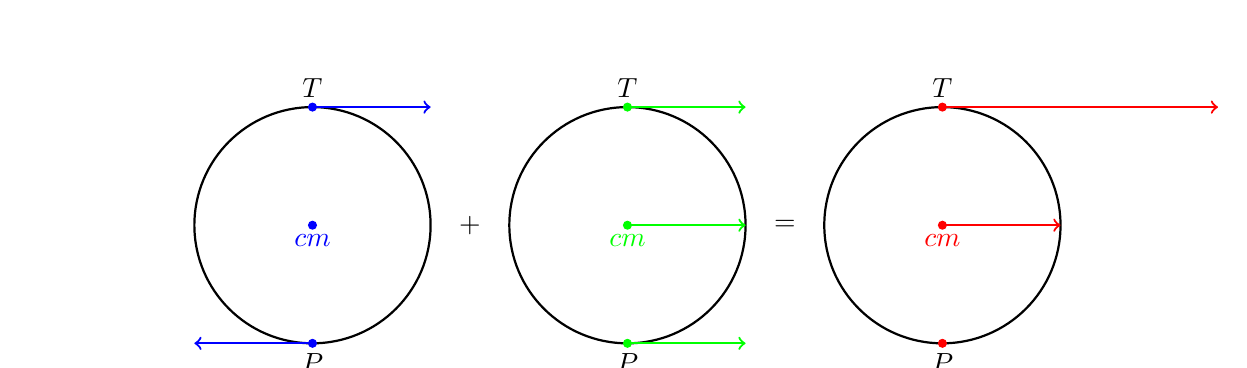
\begin{tikzpicture}
        \node at (-7.5, 0) {};

        \draw[thick] (-4, 0) circle (1.5);
        \draw[thick, ->, blue] (-4, 1.5) -- (-2.5, 1.5);
        \filldraw[blue] (-4, 1.5) circle (0.05);
        \node[anchor=south] at (-4, 1.5) {$T$};

        \filldraw[blue] (-4, 0) circle (0.05) node[anchor=north] {$cm$};

        \draw[thick, ->, blue] (-4, -1.5) -- (-5.5, -1.5);
        \filldraw[blue] (-4, -1.5) circle (0.05);
        \node[anchor=north] at (-4, -1.5) {$P$};

        \node at (-2, 0) {$+$};

        \draw[thick] (0, 0) circle (1.5);

        \draw[thick, ->, green] (0, 1.5) -- (1.5, 1.5);
        \filldraw[green] (0, 1.5) circle (0.05);
        \node[anchor=south] at (0, 1.5) {$T$};

        \draw[thick, ->, green] (0, 0) -- (1.5, 0);
        \filldraw[green] (0, 0) circle (0.05) node[anchor=north] {$cm$};

        \draw[thick, ->, green] (0, -1.5) -- (1.5, -1.5);
        \filldraw[green] (0, -1.5) circle (0.05);
        \node[anchor=north] at (0, -1.5) {$P$};

        \node at (2, 0) {$=$};

        \draw[thick] (4, 0) circle (1.5);

        \draw[thick, ->, red] (4, 1.5) -- (7.5, 1.5);
        \filldraw[red] (4, 1.5) circle (0.05);
        \node[anchor=south] at (4, 1.5) {$T$};

        \draw[thick, ->, red] (4, 0) -- (5.5, 0);
        \filldraw[red] (4, 0) circle (0.05) node[anchor=north] {$cm$};

        \filldraw[red] (4, -1.5) circle (0.05);
        \node[anchor=north] at (4, -1.5) {$P$};
    \end{tikzpicture}

    \caption{Constructing rolling without slipping motion from pure rotation and pure translation.}
    \label{fig:rolling-without-slipping}
\end{figure}

We can obtain this kind of motion by \say{summing} a pure rotation and a pure translation:
\begin{itemize}
    \item In the pure rotation $v_{\text{cm}} = 0$, $v_{P} = - \omega R \hat x$ and $v_{T} = \omega R \hat x$.
    \item In the pure translation $v_{\text{cm}} = v_{P} = v_{T} = \omega R \hat x$.
\end{itemize}
then by summing the two motions we get that $v_{\text{cm}} = \omega R \hat x$, $v_{P} = 0$ and $v_{T} = 2 \omega R \hat x$.

We can also calculate the total kinetic energy using the parallel axis theorem \ref{thm:parallel_axis}:
\begin{align}
    K & = \frac{1}{2} I_{\text{cm}} \omega^2 + \frac{1}{2} M v_{\text{cm}}^2 \\
      & = \frac{1}{2} M \omega^2 R^2 + \frac{1}{2} \frac{M R^2}{2} \omega^2  \\
      & = \frac{1}{2} \frac{3M R^2}{2} \omega^2                              \\
      & = \frac{1}{2} I_{\text{edge}} \omega^2
\end{align}
where the first $I_{\text{cm}}$ is the inertia of a disk and the second $I_{\text{edge}}$ is the inertia of a disk, that is, the edge of the wheel.

This is an interesting result because it tells us that we can view the translation-rotation motion as a pure rotation motion around the point of contact $P$ between the wheel and the ground.

\subsection{Angular momentum}

We have defined the angular momentum as $L = I \omega$. We can also define the torque as $\tau = \dv{L}{t}$.

If we consider a system where $\tau = 0$ we have that since $\tau = \dv{L}{t}$ the momentum $L$ is constant.

\begin{example}
    Consider two disks with inertia $I_1$ and $I_2$ and angular velocities $\omega_1 \ne 0$ and $\omega_2 = 0$, both of them have a stick going through their centers and they are free to rotate around the stick.
    Disk 2 touches disk 1 and they start rotating together around the stick.

    We can calculate the final angular velocity $\omega$ of the system as follows:
    \begin{align}
        I_1 \omega_1 + \cancel{I_2 \omega_2} & = (I_1 + I_2) \omega             \\
        \omega                               & = \frac{I_1 \omega_1}{I_1 + I_2}
    \end{align}
\end{example}

\begin{example}[ice skater]
    An ice skater is spinning with her arms outstretched, then she pulls her arms in.
    We want to calculate how does her angular velocity change.

    The difference between the two positions causes the moment of inertia to change because the mass is less spread out.
    Let $I_1$ be the moment of inertia with the arms outstretched and $I_2 = \frac{1}{2} I_1$ the moment of inertia with the arms pulled in and applying the conservation of momentum we get $\omega_2 = 2 \omega_1$.

    Moreover, we can calculate the kinetic energy of the system as
    \begin{equation}
        K_2 = \frac{1}{2} I_2 \omega_2^2 = \frac{1}{2} \left(\frac{1}{2} I_1\right) (2 \omega_1)^2 = 2 K_1
    \end{equation}

    This additional energy comes from the fact that the skater has to do work to pull her arms in.
\end{example}

When applying conservation of momentum choosing the right point to calculate the moment of inertia is crucial.
In fact, it is possible to have systems where the torque is zero only if we choose the right reference frame, usually choosing the center of mass as the origin of such reference frame is a good guess.

% Class of 27/03/2024

\subsection{Tensor of inertia}

\begin{figure}[H]
    \centering
    \includesvg[width=0.5\textwidth]{assets/S2_P2_PHY1/skew.svg}
    \caption{A system where the angular momentum is not parallel to the angular velocity.}
    \label{fig:tensor-of-inertia}
\end{figure}

We can write the angular velocity as $\vec{\omega} = \vec{r} \times \vec{v}$, then in this case we have $\hat \omega = \hat z$.

We can calculate the momentum as
\begin{equation}
    \abs{\vec L} = \abs{\vec{L}_{\text{top}} + \vec{L}_{\text{bottom}}} = dmv = md\omega R
\end{equation}
then
\begin{align}
    L_z & = L \cos \alpha = L \sin \theta                       \\
        & = md\omega R \sin \theta                              \\
        & = 2 m \omega R \left( \frac{d}{2} \sin \theta \right) \\
        & = 2m R^2 \omega
\end{align}

We see that in this case $\vec{L}$ and $\vec{\omega}$ don't point in the same direction.

This is because $I$ is not just a scalar but we have to specify it for all the three directions, expressing it as a matrix:
\begin{equation}
    I = \begin{pmatrix}
        I_{xx} & I_{xy} & I_{xz} \\
        I_{yx} & I_{yy} & I_{yz} \\
        I_{zx} & I_{zy} & I_{zz}
    \end{pmatrix}
\end{equation}
this matrix is symmetric, that is $I_{ij} = I_{ji}$. We call this matrix \emph{tensor of inertia}.

In order to compute the elements of the matrix it can be shown that
\begin{equation}
    \begin{cases}
        I_{zz} = \sum_i m_i (x_i^2 + y_i^2) \\
        I_{yz} = - \sum_i m_i x_i y_i       \\
        I_{xz} = - \sum_i m_i x_i z_i       \\
    \end{cases}
\end{equation}
and for $\vec{L}$ we have
\begin{equation}
    \vec{L} = \begin{pmatrix}
        L_x \\
        L_y \\
        L_z
    \end{pmatrix}
    =
    \begin{pmatrix}
        I_{xz} \omega \\
        I_{yz} \omega \\
        I_{zz} \omega
    \end{pmatrix}
\end{equation}

With some linear algebra sorcery (spectral theorem), it is possible to show that it is always possible to find such a reference frame where the tensor of inertia is diagonal and the angular momentum is parallel to the angular velocity for any object.
This only happens when the object is rotating around one of its principal axes (one of its axes of symmetry).

% Class of ???

\subsection{Static equilibrium}

We say that a system is in static equilibrium when we have the following conditions:
\begin{align}
    \sum F    & = ma = 0        \\
    \sum \tau & = \dv{L}{t} = 0 \\
    L         & = 0
\end{align}
that is, the sum of the forces is $0$, the sum of the torques is $0$, and the angular momentum (and therefore the angular velocity) is also $0$.

\subsubsection{The seesaw}

Consider the example of a seesaw with two kids of mass $m_1$ and $m_2$.
We have that
\begin{align}
    0                 & = 0 \quad \text{on the $x$ axis} \\
    N + m_1 g + m_2 g & = 0 \quad \text{on the $y$ axis}
\end{align}
where $N$ is the normal force exerted by the pivot.

We now want to add the fact that the seesaw is not rotating, but where should we compute the torque?
Since it is not rotating around any axis we could write an infinite amount of equations which all equate the torque to $0$ around some axis.
We need to show that all these possible equations are equivalent.

We can write the equation of the equilibrium for the torque as
\begin{equation}
    \tau = \sum_i \tau_i = \sum_i F_{i \perp} x_i = 0
\end{equation}
in a different axis the equation will be
\begin{equation}
    \tau' = \sum_i F_{i \perp} (x_i - d) = \sum_i F_{i \perp} x_i - d \sum_i F_{i \perp} = 0 + 0
\end{equation}

In our example a good point to pivot around would be the center of the seesaw, the point where $N$ is acting.
This allows us to drop $N$ from the equation fo the torque since $r_N = 0$.
In general it is a good choice to pivot around some point where an unknown force is acting, because then the unknown force will not contribute to the torque.

We get, in our example
\begin{equation}
    m_1 g x_1 + m_2 g x_2 = 0
\end{equation}

\section{Fluids}

In this section we will not introduce any new law, we will derive everything from Newton's laws.

\subsection{Introduction}

\subsubsection{Fields}

We will need to use a mathematical tool called field.
A field $\Phi$ is a function of space and time, that is $\Phi(\vec{r}, t)$.
Moreover this function could return a scalar as well as a vector; in this second case we call it a \emph{vector field}.

\subsubsection{Definition of fluid}

Remember the four states of matter:
\begin{itemize}
    \item Solid
    \item Liquid
    \item Gas
    \item Plasma
\end{itemize}
fluids are in the state of liquid and gas.
Remember also that the difference between liquids and gasses is that liquids are (almost) incompressible.

Also note that fluids deform continuously under the effect of any sheer force, that is, forces parallel to the area.

The surface of a liquid will try to stay at an equipotential line. We can see this phenomena in tides for example.

\subsubsection{Density}

The density a field defined as the ratio between the mass and the volume at a certain point.
\begin{equation}
    \rho(\vec r) = \dv{m}{V}
\end{equation}
Note that this is the result of a limiting process: we look at a ball centered at $\vec r$ and take the limit as the radius of the ball goes to $0$.
Also note that this assumes that the molecules are \say{continuous}, because otherwise we could get to some point where we are calculating the density of empty space.

\begin{table}[H]
    \centering
    \begin{tabular}{|c|c|}
        \hline
        \textbf{Element} & \textbf{Density}                         \\
        \hline
        Water            & $1000 \si{\kilogram \per \meter \cubed}$ \\
        Air              & $1.2 \si{\kilogram \per \meter \cubed}$  \\
        \hline
    \end{tabular}
    \caption{Common densities}
\end{table}

\subsubsection{Pressure}

The pressure is defined as
\begin{equation}
    p = \frac{F}{A}
\end{equation}
where $F$ is the component of the force $\vec{F}$ perpendicular to the area $A$.

In the context of a fluid we define the pressure in a point $\vec r$ inside a fluid as the pressure that the fluid would apply to fill an hypothetical empty ball centered at $\vec r$.
This is also a limiting process as we want to consider smaller and smaller balls.

The unit of pressure is
\begin{equation}
    [p] = \si{\kilogram \per \second \squared \per \meter} = \si {\newton \per \meter \squared} = \si{\pascal}
\end{equation}

\subsection{Stevino's law}

Consider a cylinder of fluid inside the fluid itself. We know that the fluid is in equilibrium.

\begin{align}
    F_x^{\text{tot}} & = m a_x = F_1 - F_2                                    \\
                     & = p (x_0, y_0, z_0) A - p (x_0 + \Delta x, y_0, z_0) A \\
                     & = 0
\end{align}
that is $p (x_0, y_0, z_0) = p (x_0 + \Delta x, y_0, z_0)$.
By repeating the argument in the $y$ direction we get that the pressure is independent of the $x$ and $y$ component.

For the $z$ axis we need to consider the gravitational force in addition to $F_1$ and $F_2$:
\begin{align}
    m a & = F_1 + F_2 + m g                           \\
        & = p(z_0) A + p(z_0 + \delta z) A - \rho V g \\
        & = 0
\end{align}
which can be written as, after simplifying the areas:
\begin{equation}
    p(z_0) = p(z_0 + \Delta z) + \rho g \Delta z
\end{equation}

This equation is written in a reference frame such that $z$ increases as we get closer to the surface of the fluid.
It is also common to see it written in the reference frame in which $z = 0$ at the surface of the fluid.

We can calculate the atmospheric pressure as
\begin{equation}
    p_\text{atm} \approx 10^5 \si{\pascal}
\end{equation}
in standard conditions, that is at sea level at $15 \si{\celsius}$.

\subsection{Pascal's law}

Assume we have a fluid in a container and we apply a force $F$ on top of it over a surface $A$.
Let $\delta p = F/A$, then the new pressure is
\begin{eqnarray}
    p'(\vec r) = p (\vec r) + \delta p
\end{eqnarray}
which means that the new pressure is applied homogeneously to the whole fluid.

\subsection{Archimedes principle (buoyancy)}

This law says that if we put a body in a fluid the force exerted by the fluid upwards is

\begin{equation}
    \vec F = \sum_{\text{surface}} \dd{\vec F}(\vec r) = pgV \hat k
\end{equation}

% TODO: Class of 12/04/24
TODO
\begin{itemize}
    \item
          Proof of Archimedes theorem using the divergence theorem,
    \item
          proof of divergence theorem in the case of a cube,
    \item
          as homework prove Bernoulli theorem.
\end{itemize}

% Class od 18/04/2024
\section{Kinetic theory of gasses}

\url{https://www.feynmanlectures.caltech.edu/}

Let us introduce the Angstrom: $1 \si{\angstrom} = 10^{-8} \si{\meter}$. This is the usual scale of things we will be dealing with.

\subsection{Particle collisions}

Lets start by rewriting the force for a particle $i$:
\begin{equation}
    \vec F^{(i)} = m \vec a^{(i)} = m \dv[2]{\vec r^{(i)}}{t} = - \vec \nabla \sum_{j \ne i} V(\vec r^{(i)} - \vec r^{(j)})
\end{equation}
where $V(\vec r)$ is the \emph{Lenard-Jones potential}:
\begin{equation}
    V(\vec r) = \frac{c_1}{r^{12}} - \frac{c_2}{r^6}
\end{equation}
the first term represents the force attracting the atoms to each other and the second term represents the force that repels the atoms when they get too close.

This approach presents some problems:
\begin{enumerate}
    \item \emph{Unfeasibility}: it is likely unfeasible to compute a sum with so many particles: in a volume of $1 \si{\liter}$ there are $\sim 10^{23}$ particles;
    \item \emph{Ineffectiveness}: the system is deterministically chaotic, which means that even small perturbations get amplified exponentially.
\end{enumerate}

Assume that atoms are \emph{hard spheres}, that is the centers of the two atoms cannot get closer than $2r$.

To compute the angle of reflection when two particles collide we fix one particle and draw a circle of $2r$ around it.
Then when another particle's center enters the circle we have a collision: we extend the radius of the first particle in the direction of the collision point and we get a perfect reflection along that axis:

\begin{figure}[H]
    \centering
    \includesvg[width=0.5\textwidth]{assets/S2_P2_PHY1/particle_collision.svg}
    \caption{Two particles colliding and the resulting angle $\alpha$}
\end{figure}

If we now consider a small perturbation $\delta \theta$ in the incoming particle's angle.
We get a small perturbation $\delta \alpha$ in the final angle, we now want to find $\delta \alpha(\delta \theta)$.
It can be proven (we did it in class, it's a lot of trigonometry) that
\begin{equation}
    \delta \alpha \sim \frac{d}{r} \delta \theta
\end{equation}
where $d$ is the mean free path of a particle, that is, the distance that a particle travels before hitting another one.

We now want to calculate the mean $d$.
We can assume that a particle when it travels occupies a cylinder of $2r \cross d$, while the total volume $V = \mathscr{N} V_\text{particle}$, but we know that $V_\text{particle} = (2r)^2 \pi d$ and we can get an estimate of $\frac{d}{r}$:
\begin{equation}
    \frac{d}{r} = \frac{V}{\mathscr{N}} \frac{1}{4 \pi r^3} \approx 10^3
\end{equation}

This is an issue because it means that $\dd{\alpha}$ is increasing at every collision and we have chaos.
This means that we are not able to apply newtonian physics in this situation because the error in the measurement will get out of hand too quickly,
instead we can use statistical physics to get an estimate of some of the properties of the system.

\subsection{Velocity}

We can now ask ourselves what is the probability that the $x$ component of the velocity falls in the interval $[v_x, v_x + \dd{v_x}]$.
We can write the velocity after $n$ collisions as
\begin{equation}
    v_x^{(n)} = v_x^{(0)} + \delta v_x^{(1)} + \delta v_x^{(2)} + \dots +\delta v_x^{(n)}
\end{equation}
which can be seen as a sum of many random variables.
Then $v_x \sim {\operatorfont Normal}(0, \sigma^2)$, that is
\begin{equation}
    p(v_x) = \frac{1}{\sqrt{2 \pi} \sigma} e^{-\frac{v_x^2}{2 \sigma^2}}
\end{equation}

Then we can apply some probability:
\begin{equation}
    \anglebraces{v_x^2} = E(X^2) = V(X) - (E(X))^2 = V(X) - 0 = \sigma^2
\end{equation}
and $\abs{v_x} = \sqrt{\anglebraces{v_x^2}} = \sigma$, which in real systems this is approximately $300 \si{\meter \per \second}$.

Now we can extend this reasoning to find the distribution of a particle being in a certain position at a certain velocity:
\begin{align}
    \rho(\vec r, \vec v) & = \rho(\vec r) \rho(v_x) \rho(v_y) \rho(v_z)                                                           \\
                         & = \frac{1}{V} \left(\frac{1}{\sqrt{2 \pi} \sigma}\right) e^{-\frac{v_x^2 + v_y^2 + v_z^2}{2 \sigma^2}}
\end{align}
this means that if we want to calculate the probability of the position and velocity being in some range we would have to compute
\begin{equation}
    P(\cdot) = \iiint_{\vec r \in \substack{[r_x, r_x']                                                             \\ [r_y, r_y'] \\ [r_z, r_z']}} \dd{V} \iiint_{\vec v \in \substack{[v_x, v_x']                                                             \\ [v_y, v_y'] \\ [v_z, v_z']}} \dd{v_x} \dd{v_y} \dd{v_z} \rho(\vec r, \vec v)
\end{equation}

\subsection{Pressure}

First we look at what is the momentum change that is caused by the collision of a particle with the wall.
That is
\begin{align}
    \delta p^\text{particle}_x & = -2 m v_x \\
    \delta p^\text{wall}_x     & = 2 m v_x
\end{align}

However we don't have to integrate over all the volume, if we consider a $\Delta t$ we can exclude all the volume where the particles are not fast enough to reach the wall in such time $\Delta t$: we call this volume $\Delta V$.

\begin{equation}
    \text{\# collision } = \mathscr{N} \int_{\Delta V} \frac{\dd{V}}{V} = \mathscr{N} \frac{1}{V} \underbrace{A v_x \Delta t}_{\Delta V}
\end{equation}

Then we can calculate the total momentum change in one direction:
\begin{align}
    \Delta p_x & = \int_0^\infty \dd{v_x} \rho(v_x) \delta p(v_x) (\text{\# collision for }v_x) \\
               & =\frac{2m \mathscr{N}}{V} A \Delta t \int_0^\infty \dd{v_x} v_x^2 \rho(v_x)    \\
\end{align}
then the pressure is
\begin{align}
    p = \frac{F}{A} = \frac{\Delta p / \Delta t}{A} = m \mathscr{N} \anglebraces{v_x^2}
\end{align}

\begin{align}
    \anglebraces{\delta p_x I(\text{collision happens})} & =
    \iiint \frac{\dd{x} \dd{y} \dd{z}}{V} I(\abs{x - L} < v_x \Delta t) \nonumber                                                                                                                                         \\
                                                         & \iiint \dd{v_x} \dd{v_y} \dd{v_z} \frac{1}{V} \left(\frac{1}{\sqrt{2 \pi} \sigma}\right) e^{-\frac{\norm{\vec v}^2}{2 \sigma^2}} 2 m v_x I(v_x > 0)            \\
                                                         & = \frac{A \Delta t}{V} 2m \underbrace{\iint  \dd{v_y} \dd{v_z} \left(\frac{1}{\sqrt{2 \pi} \sigma}\right) e^{-\frac{v_y^2 + v_z^2}{2 \sigma^2}}}_{1} \nonumber \\
                                                         & \underbrace{\int_0^\infty \dd{v_x} \left(\frac{1}{\sqrt{2 \pi} \sigma}\right) e^{-\frac{v_x^2 }{2 \sigma^2}}v_x^2}_{\frac{1}{2} \anglebraces{v_x^2}}           \\
                                                         & = \frac{m A \Delta t}{V} \anglebraces{v_x^2}
\end{align}

Then the total momentum shift is
\begin{equation}
    \Delta p_x = \mathscr{N} \frac{m A \Delta t}{V} \anglebraces{v_x^2}
\end{equation}
and we can calculate the pressure as
\begin{align}
    p & = \frac{F_x}{A} = \frac{\Delta p_x / \Delta t}{A}          \\
      & = \mathscr{N} \frac{m}{V} \anglebraces{v_x^2}              \\
      & = \frac{2 \mathscr{N}}{V} \anglebraces{\frac{1}{2}m v_x^2} \\
      & = \frac{2 \mathscr{N}}{3 V} \anglebraces{\frac{1}{2}m v^2} \\
      & = \frac{2 \mathscr{N}}{3 V} U
\end{align}
where $U$ is the internal energy. We then get the famous relationship
\begin{equation}
    \label{eq:gas:internal_energy}
    pV = \frac{2}{3}U
\end{equation}

\section{Thermodynamics}

If we consider a moving box with some gas inside we can write the velocity of a particle as
\begin{equation}
    \vec v^{\text{(particle)}} = \vec c_{\text{CM}} + \vec u
\end{equation}
where $\vec u$ is the maxwell-distributed velocity relative to the center of mass.
Moreover we can write the energy for $\mathscr{N}$ particles as
\begin{equation}
    E = \frac{1}{2} \mathscr{N} m v_{\text{CM}}^2 + U
\end{equation}

Thermodynamics is all about converting macroscopic energies (like kinetic energy, potential energy, or work) to microscopic energies (like internal energy or thermal agitation).

This internal energy can be transferred, we call this \emph{energy in motion} \textbf{heat}.
Heat can be transferred in three main ways: conduction, convection and radiation.
For example, if we put together a hot and a cold container after a while they will reach thermal equilibrium, that is the macroscopic observables do not change anymore.
This is an example of conduction, which is the way of transferring heat we will focus on.

\subsection{Temperature}

Consider an isolated system with $\mathscr{N}_1$ particles of mass $m_1$ and $\mathscr{N}_2$ particles of mass $m_2$.
Both gasses start in equilibrium within themselves at time $(i)$ and they are combined together.
At time $(f)$ the combined gasses reach equilibrium with each other.

Since the system is isolated the energy is conserved:
\begin{equation}
    U_1^{(i)} + U_2^{(i)} = U_1^{(f)} + U_2^{(f)}
\end{equation}
which we can write as
\begin{equation}
    \mathscr{N}_1 \anglebraces{\frac{1}{2} m_1 v^2}_{\sigma_1^{(i)}} + \mathscr{N}_2 \anglebraces{\frac{1}{2} m_2 v^2}_{\sigma_2^{(i)}} = \mathscr{N}_1 \anglebraces{\frac{1}{2} m_1 v^2}_{\sigma_1^{(f)}} + \mathscr{N}_2 \anglebraces{\frac{1}{2} m_2 v^2}_{\sigma_2^{(f)}}
\end{equation}
and simplifying we get
\begin{equation}
    \mathscr{N}_1 m_1 \left(\sigma_1^{(i)}\right)^2 + \mathscr{N}_2 m_2 \left(\sigma_2^{(i)}\right)^2 = \mathscr{N}_1 m_1 \left(\sigma_1^{(f)}\right)^2 + \mathscr{N}_2 m_2 \left(\sigma_2^{(f)}\right)^2
\end{equation}

By this equation we get that at time $(t)$ the $\sigma$ have changed.

By conducting an experiment we can note the following fact
\begin{equation}
    \frac{p_1 V_1}{\mathscr{N}_1} = \frac{p_2 V_2}{\mathscr{N}_2}
\end{equation}
and by substituting \autoref{eq:gas:internal_energy} we get that
\begin{equation}
    m_1 \left( \sigma_1^{(f)} \right) = m_2 \left(\sigma_2^{(f)}\right) = K_b T
\end{equation}
where $K_B = 1.38 \cdot 10^{-23} \si{\joule \per \kelvin}$ is the Boltzmann constant and $T$ is the temperature, measured in kelvin ($\si{\kelvin}$).

We can now explicit the pdf of the velocity:
\begin{equation}
    \rho(\vec v) = \frac{\sqrt{m}}{\sqrt{2 \pi K_b T}} e^{- \frac{m v^2}{2 K_B T}}
\end{equation}
and we can write
\begin{equation}
    \label{eq:gas:initial_perfect}
    p V = \frac{2}{3}U = \frac{2}{3}\mathscr{N} \anglebraces{\frac{1}{2}mv^2} = \mathscr{N}K_B T
\end{equation}
but $\mathscr{N}$ is very big and $K_B$ is very small, so we can define a few more things to make this better.

The Avogadro number $N_A$ is the number of atoms of hydrogen in $1 \si{\gram}$ and it is equal to $N_A = 6.02 \cdot 10^{23}$ (pure number).
Moreover we define $1 \si{\mole}$ of some gas as $1 \cdot N_A$ of this gas.

Then we can write \autoref{eq:gas:initial_perfect} as
\begin{equation}
    pV = n \underbrace{N_A K_B}_{\text{constant } = R} T
\end{equation}
where we noted that $N_A K_B$ are both constant, therefore we can define the constant of ideal gasses as $R = 8.32 \si{\joule \per \kelvin}$ and we write the law of perfect gasses in the final form:
\begin{equation}
    \label{eq:gas:perfect}
    pV = nRT
\end{equation}

\subsubsection{Unit of measure of temperature}

We measure the temperature in $\si{\kelvin}$ where $0 \si{\celsius} = 273.15 \si{\kelvin}$.
The celsius is a more historical unit that was measured by looking at the phase shift points of water at $1 \si{\atm}$ which is a quite reliable way to measure temperature.

We chose the $0 \si{\kelvin}$ to be where it is because at that temperature all gasses have so little kinetic energy that they basically don't move anymore and create no pressure.

\subsection{Transformations}

\subsubsection{Reversible adiabatic compression}

We compress the gas of some $\dd{V} < 0$ very slowly such that at every step we give the gas the time to reach a well defined maxwell distribution.
In this way the gas does not lose energy.

We will call $W$ the work done \emph{on} the gas and we have that $\dd{W} = \dd{U}$.
Moreover the work done on the gas can also be written as
\begin{equation}
    \dd{W} = F \dd{x} = p A \dd{x} = p \dd{V}
\end{equation}

Differentiating \autoref{eq:gas:internal_energy} we get
\begin{equation}
    \dd{U} = \frac{3}{2} (\dd{p} V + p \dd{V}) = -p\dd{V}
\end{equation}
which we can arrange as
\begin{equation}
    \frac{\dd{p}}{p} + \frac{5}{3}\frac{\dd{V}}{{V}} = 0
\end{equation}
which is separable differential equation which we can solve to get
\begin{equation}
    \dd{\log p} + \frac{5}{3} \dd{\log V} = 0
\end{equation}
but this means that if we collect the $\dd$ we obtain that the rest must be constant because the derivative is $0$.
We get that
\begin{equation}
    p V^\gamma = \text{ const}
\end{equation}
where $\gamma = \frac{5}{3}$ if we assume the gas is monoatomic.

Moreover, somehow the following relationship holds
\begin{equation}
    pV = (\gamma - 1) U
\end{equation}

\subsubsection{Isothermic compression}

In this transformation the temperature of the gas is constant.
To do this we use a thermal reservoir whose temperature is always $T$ and we move the piston slow enough such that the temperature is always in equilibrium.

We start by defining the work done by the piston:
\begin{equation}
    \dd{W} = - p \dd{V}
\end{equation}
and the total work will be
\begin{equation}
    W = \int_\text{initial}^\text{final} \dd{W} = \int_{V_i}^{V_f} p(V) \dd{V} = -nRT \int_{V_i}^{V_f} \frac{\dd{V}}{V} = n R T \log \frac{V_i}{V_f}
\end{equation}
where we applied \autoref{eq:gas:perfect}.

Moreover, note that the work we are doing on the gas is \say{leaking} to the reservoir, that is the gas is releasing some heat $Q$.

We can now define the first principle of thermodynamics:
\begin{equation}
    \label{eq:gas:first_principle}
    \Delta U = W + Q
\end{equation}

Since in this transformation $\Delta U = 0$ we have that $W = -Q$.

\subsubsection{Isocloric transformation}

We keep the volume the same and change the temperature and pressure.

Since the volume is constant there is no work being done by the gas, therefore all the heat goes into the internal energy, according to \autoref{eq:gas:first_principle}.

In the case of ideal gasses we will have that
\begin{equation}
    Q = \frac{3}{2}nR\Delta T
\end{equation}

\subsubsection{Isobaric transformation}

The property of this transformation is that $p_A = p_B$. We can apply \autoref{eq:gas:perfect} and \autoref{eq:gas:first_principle} to get the heat.

First we can write the difference of internal energy as
\begin{equation}
    \Delta U = \frac{3}{2}n R (T_B -T_A)
\end{equation}
and the work will be
\begin{equation}
    \dd{W} = -p \dd{V} \implies W = -p (V_B - V_A)
\end{equation}
but we also know that $pV = nRT$, which means we can write
\begin{equation}
    W = -nR (T_B - T_A)
\end{equation}
then the heat then will be
\begin{equation}
    Q = \frac{5}{2}nR(T_B - T_A)
\end{equation}

Moreover, by applying the ideal law of gasses to the whole transformation we get
\begin{equation}
    \frac{V_A}{T_A} = \frac{V_B}{T_B}
\end{equation}

\subsubsection{Summary}

\begin{table}[H]
    \centering
    \renewcommand{\arraystretch}{2}
    \begin{tabular}{|c||c|c|c|c|}
        \hline
        \textbf{Transformation} & \textbf{Property}                                         & $\bm{\Delta U}$          & $\bm{W}$                   & $\bm{Q}$                  \\
        \hline
        Reversible Adiabatic    & $Q = 0 \implies p_A V_A^\gamma = p_B V_B^\gamma$          & $\frac{3}{2}nR\Delta T$  & $\frac{3}{2}nR\Delta T$    & $0$                       \\
        Irreversible Adiabatic  & $Q = 0$                                                   &$\frac{3}{2}nR\Delta T$&$-p\Delta V$& $0$                       \\
        Isothermal              & $\Delta T = 0 \implies p_A V_A = p_B V_B$                 & $0$                      & $-nRT\log \frac{V_B}{V_A}$ & $nRT\log \frac{V_B}{V_A}$ \\
        Isocloric               & $\Delta V = 0 \implies \frac{p_A}{T_A} = \frac{p_B}{T_B}$ & $\frac{3}{2}nR\Delta T$  & $0$                        & $\frac{3}{2}nR\Delta T$   \\
        Isobaric                & $\Delta p = 0 \implies \frac{V_A}{T_A} = \frac{V_B}{T_B}$ & $\frac{3}{2}nR \Delta T$ & $-nR \Delta T$             & $\frac{5}{2}nR \Delta T$  \\
        \hline
    \end{tabular}
    \caption{Summary of the main transformations}
\end{table}

\subsection{Heat}

\subsubsection{Specific heat}

We want to extend the relationship between heat and temperature.
We already saw the following relationships:
\begin{align}
    pV & = (\gamma - 1)U \\
    pV & = nRT
\end{align}
where $\gamma$ depends on the gas and in the case of a monoatomic ideal gas $\gamma = 5/3$.

If we put these two relationships together we get
\begin{equation}
    \label{eq:gas:internal_energy_2}
    U = \frac{3}{2}nRT
\end{equation}

Now consider \autoref{eq:gas:first_principle} where $W = 0$, which means $\Delta U = Q$ and combining with \autoref{eq:gas:internal_energy_2} we get
\begin{equation}
    \Delta U = Q = \underbrace{\left(\frac{3}{2} n R \right)}_{C_H} \Delta T
\end{equation}
where $C_H$ is the specific heat: in the case of ideal monoatomic gasses it is the one written in the equation but for other gasses it can change.

Note that this quantity depends on the amount of gas we have, we can therefore define the specific heat $C$ and the molar specific heat.
\begin{equation}
    C = \frac{C_H}{m} = \si{\joule \per \kelvin \per \kilogram}
\end{equation}

Moreover we define the calorie ($1 \si{\calorie}$) as the heat necessary to raise from $14.5 \si{\celsius}$ to $15.5 \si{\celsius}$ $1 \si{\gram}$ of water.

\subsubsection{Latent heat}
When a substance changes state, during the phase transition all the energy goes into the phase transition itself without raising the temperature of the substance.
The energy needed for the full phase transition is dependent on the mass and we write it as
\begin{equation}
    \delta Q = L m
\end{equation}
where $L$ is the latent heat which depends on the substance itself; it is measured in $\si{\joule \per \kilogram}$.

\subsubsection{State variables}

Consider two transformations $A$ and $B$:
\begin{figure}[H]
    \centering
    \includesvg[width=0.75\textwidth]{assets/S2_P2_PHY1/work_in_transformation.svg}
    \caption{Two transformations $A$ and $B$}
\end{figure}

Before we computed the work as $\int p \dd{V}$ but note that this integral is not path independent: if we choose a different transformation we will get a different result.

We have that $\dd{U}$ is path independent but $\delta W$ and $\delta Q$ are not, therefore we can have a system that goes back to the original state but can still do work.

\subsection{Irreversibility}

Consider a container divided by a wall where all the particles are all on one side of the wall. Now open a little hole on the wall: the particles will distribute between the two parts of the container.

In theory there is nothing preventing the particles to go back to the initial position all in the same side of the wall, but this is so unlikely that it never happens.

We have that each microstate (that is the exact position and velocity of the particles) are equally likely, but some macrostates (that is the amount of particles in each side) are much much much more likely than others.

If you sort a deck of cards and then you shuffle it the probability of it being sorted after some time is so low that it actually never happens.
But if instead the deck is made of just 2 cards and we shuffle them the probability that they stay sorted is actually $1/2$.

The same happens with particles:
the likelihood of a macrostate to happen is dependent on the number of particles in the system.

\subsection{Entropy}

This is another state variable which depends just on the state of the system.
We do not prove it exist, entropy is postulated as follows:

\begin{definition}[entropy]
    For any thermodynamic process $p: i \to f$ where $i$ is the initial state and $f$ is the final state. We have that the difference in entropy between the two states is
    \begin{equation}
        \Delta S = \int_i^t \frac{\dd{Q}}{T} = S_f - S_i
    \end{equation}
    where $S$ is path independent.

    Note that the thermodynamic process $p$ must be reversible otherwise we wouldn't have a function to describe it and wouldn't be able to take the integral.
\end{definition}

\begin{example}
    Consider a transformation of an ideal gas.
    We know that $\dd{U} = \delta W + \delta Q$, but we also know that $\dd{U} = \frac{3}{2} n R \dd{T}$ and $\delta W = -p \dd{V}$.
    Then we can write $\delta Q = \dd{U} - \delta W$.
    We can compute the entropy by using $pV = nRT$ as
    \begin{align}
        \Delta S & = \int_i^t \frac{\frac{3}{2} n R \dd{T}}{T} + \int_i^t \frac{p \dd{V}}{T}                   \\
                 & = \frac{3}{2} nR \log \frac{T_f}{T_i} + \int_i^t \frac{(nR\cancel{T}/V) \dd{V}}{\cancel{T}} \\
                 & = \frac{3}{2} nR \log \frac{T_f}{T_i} + nR \log \frac{V_f}{V_i}
    \end{align}
    which is indeed a state variable.
\end{example}

Now that we saw that this works for ideal gasses we postulate that this also works for real cases:

\begin{theorem}[second principle of thermodynamics]
    \label{thm:gas:second_principle}
    In a closed system if we apply a thermodynamic process $p: i \to f$ we will have that
    \begin{equation}
        \Delta S \geq 0
    \end{equation}
    and if $\Delta S = 0$ then the process is reversible.
\end{theorem}

\begin{example}[isothermal expasion]
    Consider an isothermal expansion where the gas goes from $V$ to $2V$ and it is in contact with a reservoir of temperature $T$.

    Since $T$ is not changing we can calculate the entropy of the gas as
    \begin{equation}
        \Delta S^{\text{(gas)}} = n R \log 2
    \end{equation}
    but from the point of view of the reservoir we will have a entropy change of $\Delta S^{\text{(reservoir)}} = - \Delta S^{\text{(gas)}}$, which confirms that isothermal transformations are reversible.
\end{example}

Boltzmann calculated the entropy of a system as
\begin{equation}
    S = K_b \log W
\end{equation}
where $W$ is the volume of the macrostate.
This basically tells us that the gasses always want to occupy as volume as possible.

\subsection{Efficiency of engines}

We define the efficiency as
\begin{equation}
    \label{eq:gas:efficiency}
    \eta = \frac{W}{Q_H}
\end{equation}
where $W$ is the work and $Q_H$ is the heat absorbed from the hot reservoir.

We will have an engine that produces work $W$ using some heat $Q_H$ and dumbing some heat $Q_C$ in some cold reservoir.
The engine will be cyclical.

We will have that the entropy change is given just by the exchange in temperature and heat in the reservoirs which is just
\begin{equation}
    \Delta S = - \frac{Q_H}{T_H} + \frac{Q_C}{T_C} \geq 0
\end{equation}
and by substituting into \autoref{eq:gas:efficiency} we get that
\begin{equation}
    \eta = \frac{Q_H - Q_C}{Q_H} = 1 - \frac{Q_C}{Q_H} \leq 1 - \frac{T_C}{T_H}
\end{equation}
which means that the efficiency is never $1$.

We can then express the second principle of thermodynamics as the Kelvin's or Clausius' principle that state respectively that there exists no engine that has $Q_C > 0$ and that a \say{perfect fridge} does not exist.

\end{document}
